\chapter{Implementation and Results}

This chapter focuses on comparing the performance between \acrshort{mcmc} and \acrshort{vi} methods for performing inference in a \acrshort{pgm}. Each method have their strengths and weaknesses for different types of problems. As a compromise, this chapter will focus on comparing the performance of a fictitious model in order to discuss a concrete example.  

\section{The model}
As the context of this paper is intention inference for autonomous ferries, it seems fit that a similar example is used. A simple intention model is therefore proposed as an example, which relates steering angle to an intention through a mixture model. 

The angle $\theta_t$ is defined to be the angle between the obstacles current course and the predicted course given the obstacles final destination. If the obstacles reported final destination is correct, $D_t=0$, the angle should be closely related to the obstacles intention and can be generated from a Gaussian selected by the intention $I_t$ (i.e. a mixture of Gaussians weighted by the intention probabilities). If the obstacle report an incorrect destination, $D=1$, the angle $\theta_t$ is independent of intention.

Whether or not the final destination is valid is modelled using a Bernoulli variable $D_t$ which takes the value $1$ if the destinations is \textbf{invalid}. A Beta distribution is used to model the prior probability of $D=1$, i.e. the destination being invalid.  

\begin{equation}
    p_D \sim \text{Beta}, \quad p_D \in (0, 1)
\end{equation}
\begin{equation}
    D_t \sim \text{Bernoulli}(p_D), \quad D_t \in \{0, 1\}
\end{equation}

The intention in a situation $I_t$ is modelled by a Categorical discrete variable where the possible realizations are shown in \cref{tbl:intentions}. The intention probabilities $\boldsymbol{\alpha}$ are distributed according to a Dirichlet distribution.

\begin{equation}
    \boldsymbol{\alpha} \sim \text{Dirichlet}, \quad \boldsymbol{\alpha} \in \{\alpha_0, \alpha_1, \alpha_2 \in (0, 1) \; | \; \sum_i \alpha_i = 1 \}
\end{equation}
\begin{equation}
    I_t \sim \text{Categorical}(\boldsymbol{\alpha}), \quad I_t \in \{0, 1, 2\}
\end{equation}

\begin{table}[h]
\centering
\begin{tabular}{|l|l|}
\hline
$I_t=0$ & The obstacle intends to keep its current course \\ \hline
$I_t=1$ & The obstacle intends a starboard turn           \\ \hline
$I_t=2$ & The obstacle intends a portside turn            \\ \hline
\end{tabular}
\caption{Possible realizations of the intention $I_t$}
\label{tbl:intentions}
\end{table}


The mixture components for $\theta_t$ when $D_t=0$ are Gaussian Distributions with unknown mean and variance. The mean and variance for component $I=i$ is 
\begin{align}
    \mu_{i} &\sim \text{Gaussian} & \sigma_i &\sim \text{Inv-Gamma}
\end{align}
When $D=0$ and $I_t=i$, the angle is distributed according to
\begin{equation}\label{eq:theta_intention_mixture}
    \theta_t^{(I=i)} \sim \mathcal{N}_{I=i}(\mu_i, \sigma_i^2), \quad \theta_t^{I=i} \in \mathcal{R}
\end{equation}

One issue with using Guassian for angle information is that the Gaussian Distribution has support on $\mathcal{R}$, while the angles $\theta$ should ideally only have support on $(-\pi, \pi)$. In practice, this may not be a big issue as long as the probability mass is mostly kept within $(-\pi, \pi)$. Another solution could be to use a nonlinear transformation to clamp $\mathcal{R}$ to $(-\pi, \pi)$.

\cref{fig:intention_angle} shows the likelihood for different angles for the different intentions with fixed mean and variance. 

When the obstacles target destination is invalid, $D=1$, the angle $\theta$ is distributed according to a Uniform distribution over the range $(-\pi, \pi)$ to model how the angle contains no information about the obstacle in such a case. 

\begin{equation}
    \theta_t^{(D=1)} \sim \text{Uniform}(-\pi, \pi)
\end{equation}


The data generating process for $\theta_t$ then becomes:

\begin{enumerate}
    \item Draw priors $p_D$, $\boldsymbol{\alpha}$ 
    \item Draw priors $\mu_i$ and $\sigma_i$ for all intentions 
    \item Draw $D_t$ and $I_t$ conditional on $p_D$ and $\boldsymbol{\alpha}$
    \item If $D_t=1$, draw $\theta_t$ from Uniform distribution. If not, draw $\theta_t$ from $\mathcal{N}_{I=i}$ conditional on $\mu_i$ and $\sigma_i$.
\end{enumerate}


\begin{figure}
    \centering
    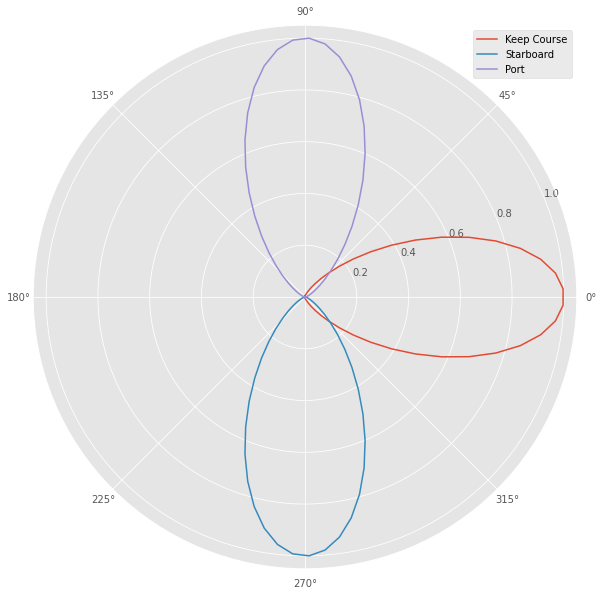
\includegraphics[width=0.8\textwidth]{figures/intention_angle.png}
    \caption{Normalized likelihood of different angles under different intention hypotheses. This is a polar plot where the angle represent $\theta_t^{(I=i)}$, the radius represent the probability. This is generated from \cref{eq:theta_intention_mixture} with $\mu_0=0$, $\mu_1 = \frac{\pi}{2}$, $\mu_2=-\frac{\pi}{2}$ and $\sigma_i=\frac{\pi}{8}$}
    \label{fig:intention_angle}
\end{figure}


\section{Dataset \& Benchmark}
\section{Markov Chain Monte Carlo}
\section{Variational Inference}